\section{Initialisation}
\label{s:Initialisation}

\subsection{Monocular Initialisation}
The monocular initialisation is a key module in the Visual-Odometry pipeline.
It is ordered in the follwoing way:
\begin{enumerate}
	\item Find the 2D-2D correspondences between the the chosen first two images
	\item Apply the 8-point Algorithm to estimate the Fundamental matrix combined with running RANSAC.
	\item Check the validity of the estimated Fundamental matrix by either comparing the reprojection error or the distance to the epipolar line. 
	\item RANSAC return a set of inlier of the current 2D-2D correspondences.
	\item With the new set of inlier we can re-evaluate the final Essential Matrix $E$ estimate.
	\item The Essential Matrix $E$ can then be decomposed into two rotation and two translation hypotheses for the pose of the first camera frame. This gives in total a set of four camera motion possibilities.
	\item These hypotheses have to be disambiguated to choose the right camera rotation and translation.
\end{enumerate}

We have implemented two different approaches for finding the 2D-2D correspondences:

\begin{enumerate}
	\item Exercise implementation of Harris descriptor and detector.
	\item Implementation of the Kanade-Lucas Tracker (KLT).
\end{enumerate}

\begin{figure}
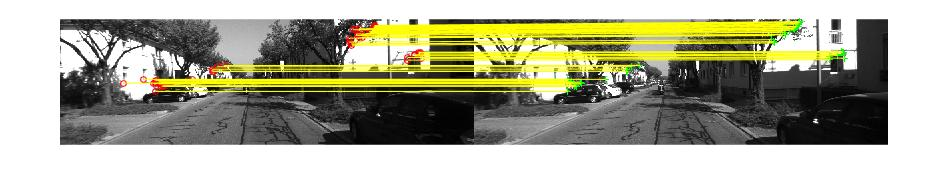
\includegraphics[width=0.98\textwidth]{files/KLT_2d2d.jpg}
\caption[\label{s:KLT_2d2d}]{2D-2D correspondences with KLT.}
\end{figure}

An examplary output of the 2D-2D module can be seen in Figure~\ref{s:KLT_2d2d}. The correspondences between two images are indicated.

Due to efficiency reasons we decided to use the epipolar line distance as a measure to validate the estimated Fundamental Matrices. In theory the reprojection error would have yielded better results (sacrificing efficiency); however, in our case the differences were neglectable.

\section{Continous Operation}
\label{s:ContOp}

\subsection{KLT}

\section{Bonus Features}
\label{s:BF}

\subsection{Plotting}

\subsection{Automatic Selection of Frames for Initialisation}

\subsection{Relocalisation}

\subsection{Full Bundle Adjustment}

\subsection{Calibrated Smartphone Camera and own Dataset}

In order to assess the robustness of our VO pipeline, we decided to record our own dataset.
For this endeavour, we printed a checkerboard to calibrate the camera of an smartphone.
We then used the calibrated camera to record the dataset.
In order to achieve good results for the calibration, we made sure that we followed the following procedure:

1) Set focus and exposure mode of the smartphone to fixed.
2) Ensure that the checkerboard is over a planar surface and presents no light reflections.
3) Take frames of the checkerboard from sufficiently different angles and distances.

Once the calibration dataset recorded, we proceeded to find the intrinsics of the camera.
As a first approach we used the matlab toolbox (REFERENCE TO THE TOOLBOX https://www.vision.caltech.edu/bouguetj/calib_doc/).
Unfortunately, we could not get good calibration results.
This was in part due to the fact that the interface requires you to click on the
corners of the checkerboard in the image, and therefore limits the amount of images you can process in a given time.
We also used OpenCV to retrieve the calibration matrix of the camera. Nonetheless, we found that the most user-friendly
calibration tool was the one offerd as a matlab app named Camera Calibrator.

Using this last tool, we managed to retrieve approximately the same intrinsic parameters independently of the calibration images.
Once calibrated, we processed the images to get a gray-scaled, resized and undistorted set of images. Then we fed the new
dataset to our VO pipeline and checked the results with our ground truth.
The ground truth was taken approximately with no special instrumentation other than a meter.

We encountered many problems while recording the dataset, to name a few: motion blur when moving, changes of illumination on the scene,
mantaining a constant focus, transferring images, having enough features on the scene, etc.

In the end, we found that monocular initialisation was having difficulties to output a sufficient amount of 2D-3D correspondences.
This led the continuous operation part to stop after two frames on average. The reprojetion errors on the triangulated keypoints were of
the order of magnitude of tens of pixels, depending on parameters and bootsrap_frames.

In the end, we learned about different tools available for camera calibration and about the difficulties of recording a satisfiable dataset
for visual odometry. Or seen from another perspective, we learned about the limits of our VO pipeline.

Our calibration files and images of the dataset are provided under the folder Smartphone.








\subsection{Quantitative Analysis}
\subsubsection{Keypoint Tracking via Block Matching versus KLT}

\subsection{Monocular Initialisation Harris Detector via Matlab versus Exercise Harris Detector}
